\chapter{Simulación del analizador descendente predictivo}

El simulador de análisis sintáctico descendente predictivo representa el núcleo tecnológico más sofisticado de SimAS 3.0, diseñado específicamente para simular y visualizar el proceso completo de análisis sintáctico de gramáticas libres de contexto utilizando el algoritmo LL(1). Este componente avanzado no solo ejecuta el análisis, sino que proporciona una experiencia educativa inmersiva que permite a los usuarios comprender profundamente los mecanismos internos del análisis sintáctico predictivo, desde la construcción de la tabla de análisis hasta la ejecución paso a paso del algoritmo.

\section{Introducción al simulador}

El simulador de SimAS 3.0 implementa un analizador descendente predictivo de última generación que utiliza una tabla de análisis precomputada para determinar de manera determinista qué producción aplicar en cada paso del análisis. Este enfoque algorítmico avanzado garantiza un análisis eficiente y completamente determinista de las cadenas de entrada, siempre que la gramática cumpla con las condiciones LL(1). La implementación incluye optimizaciones específicas para el manejo de gramáticas complejas y sistemas de recuperación de errores robustos que mejoran significativamente la experiencia del usuario.

\subsection{Características principales}

El simulador incorpora un conjunto integral de funcionalidades avanzadas que lo convierten en una herramienta educativa y profesional de primer nivel:

\begin{itemize}
    \item \textbf{Asistente guiado inteligente}: proceso de configuración estructurado en 5 pasos secuenciales con validación automática en tiempo real y retroalimentación inmediata sobre la corrección de cada transformación.
    \item \textbf{Refactorización automática avanzada}: eliminación sistemática de recursividad izquierda directa e indirecta, factorización de producciones con prefijos comunes, y optimización de la estructura gramatical para análisis LL(1).
    \item \textbf{Cálculo de conjuntos PRIMERO y SIGUIENTE}: generación automática y eficiente de los conjuntos fundamentales utilizando algoritmos optimizados que manejan gramáticas de cualquier complejidad.
    \item \textbf{Construcción de tabla predictiva}: generación automática de la tabla de análisis LL(1) con detección de conflictos y sugerencias de resolución.
    \item \textbf{Sistema de funciones de error}: implementación de un sistema avanzado de recuperación de errores con funciones predefinidas y capacidad de personalización completa.
    \item \textbf{Simulación interactiva completa}: análisis paso a paso con control granular del usuario, incluyendo avance, retroceso, pausa y reinicio en cualquier momento del proceso.
    \item \textbf{Visualización dinámica}: generación automática de derivaciones en formato BNF y árboles sintácticos que se actualizan en tiempo real durante la simulación.
    \item \textbf{Múltiples simulaciones concurrentes}: capacidad de ejecutar y gestionar múltiples simulaciones simultáneamente para análisis comparativo y validación exhaustiva.
\end{itemize}

\section{Acceso al simulador}

El simulador está diseñado con múltiples puntos de acceso estratégicos que facilitan su uso en diferentes contextos de trabajo, optimizando el flujo de trabajo del usuario:

\subsection{Desde el menú principal}

El acceso principal al simulador se realiza a través de la interfaz principal de la aplicación:

\begin{itemize}
    \item \textbf{Menú \string"Simulador\string"}: acceso directo e inmediato al simulador principal, ideal para usuarios que desean comenzar una nueva simulación desde cero.
    \item \textbf{Atajo de teclado \string"Ctrl + S\string"}: acceso rápido mediante combinación de teclas para usuarios experimentados que prefieren la eficiencia del teclado.
\end{itemize}

\subsection{Desde el editor de gramáticas}

La integración con el editor proporciona una transición fluida y contextual:

\begin{itemize}
    \item \textbf{Botón \string"Simular\string"}: disponible únicamente cuando hay una gramática válida cargada en el editor, garantizando que el usuario siempre trabaje con gramáticas correctas y completas.
\end{itemize}

Esta integración asegura que la gramática editada se transfiera automáticamente al simulador, manteniendo la consistencia y evitando errores de configuración.

\section{Asistente guiado del simulador}

El asistente del simulador representa una innovación en la experiencia de usuario, diseñado para guiar de manera intuitiva y educativa a través de un proceso estructurado de 5 pasos que transforma una gramática libre de contexto en un sistema de análisis sintáctico completamente funcional. Cada paso está cuidadosamente diseñado para realizar transformaciones específicas y cálculos fundamentales, proporcionando al usuario una comprensión profunda de cada etapa del proceso.

\subsection{Navegación del asistente}

El asistente incorpora un sistema de navegación sofisticado que maximiza la usabilidad y el control del usuario:

\begin{itemize}
    \item \textbf{Navegación bidireccional}: botones \string"Anterior\string" y \string"Siguiente\string" permiten moverse libremente entre los pasos, facilitando la revisión y corrección de configuraciones previas.
    \item \textbf{Acceso a la gramática original}: el botón \string"Gramática\string" está disponible en el menú inferior de todos los pasos, proporcionando acceso inmediato a la gramática original sin refactorizar ni eliminar recursividad, como se puede observar en la figura \ref{fig:gramatica_original}. Esta funcionalidad es crucial para comparar el estado original con las transformaciones aplicadas.
    \item \textbf{Validación automática en tiempo real}: cada paso implementa un sistema de validación automática que verifica la corrección de los resultados antes de permitir continuar, garantizando la integridad del proceso y proporcionando retroalimentación inmediata.
\end{itemize}

\needspace{8cm}
\begin{figure}[H]
    \centering
    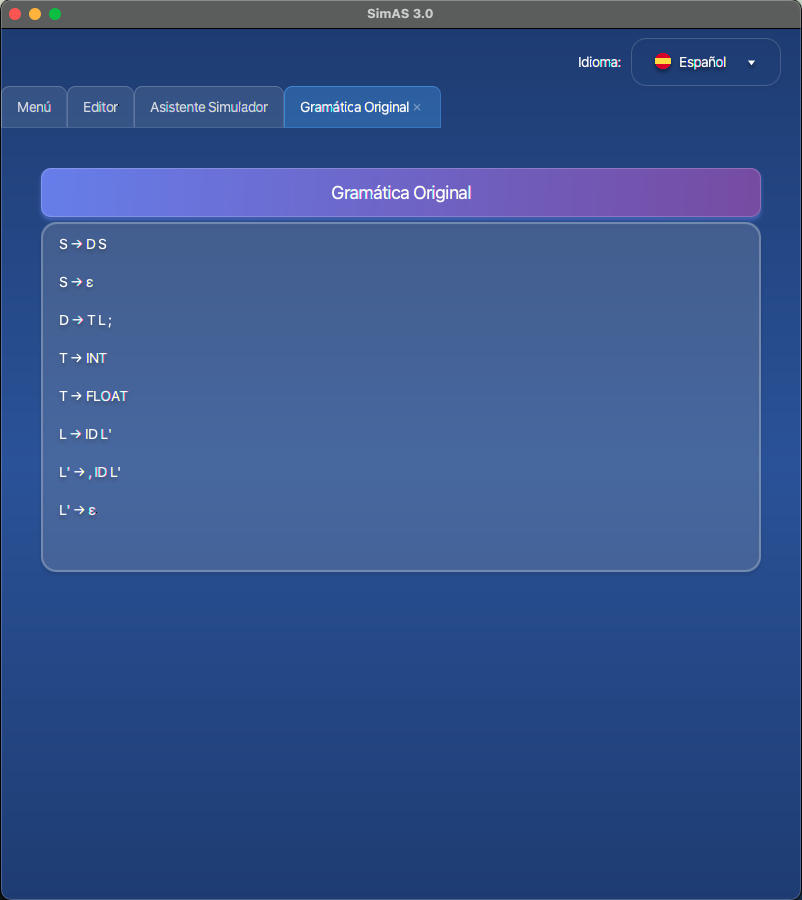
\includegraphics[width=0.9\textwidth]{figuras/simulador/gramatica_original.png}
    \caption{Vista de la gramática original desde el botón \string"Gramática\string".}
    \label{fig:gramatica_original}
\end{figure}

\subsection{Paso 1: Refactorización y eliminación de recursividad}

El primer paso del asistente constituye la fase más crítica del proceso, donde el simulador procesa la gramática original aplicando transformaciones algorítmicas avanzadas para prepararla adecuadamente para el análisis LL(1). Este paso es fundamental porque determina la viabilidad del análisis predictivo y establece las bases para todos los cálculos posteriores.

\subsubsection{Procesos realizados}

El simulador ejecuta una secuencia de algoritmos especializados:

\begin{itemize}
    \item \textbf{Eliminación de recursividad izquierda}: implementa algoritmos avanzados que detectan y eliminan tanto recursividad directa como indirecta, transformando la gramática en una forma equivalente que no presenta este problema estructural.
    \item \textbf{Factorización de producciones}: aplica técnicas de factorización para identificar y resolver producciones con prefijos comunes, eliminando ambigüedades que podrían causar conflictos en la tabla predictiva.
    \item \textbf{Validación LL(1)}: ejecuta un análisis exhaustivo para verificar que la gramática resultante cumple con todas las condiciones necesarias para ser LL(1), incluyendo la ausencia de conflictos en la tabla predictiva.
\end{itemize}

\subsubsection{Interfaz del paso 1}

La interfaz del primer paso, ilustrada en la figura \ref{fig:paso1_refactorizacion}, presenta una vista comprensiva del proceso de transformación:

\begin{itemize}
    \item \textbf{Gramática refactorizada}: muestra la gramática completamente transformada con todas las modificaciones aplicadas, permitiendo al usuario verificar la corrección de las transformaciones.
    \item \textbf{Estado de la gramática}: proporciona indicadores visuales claros sobre la validez y completitud de la gramática, incluyendo métricas de calidad y advertencias sobre posibles problemas.
    \item \textbf{Detalles de transformaciones}: presenta información detallada sobre cada cambio realizado, incluyendo el tipo de transformación aplicada y su justificación algorítmica.
\end{itemize}

\needspace{8cm}
\begin{figure}[H]
    \centering
    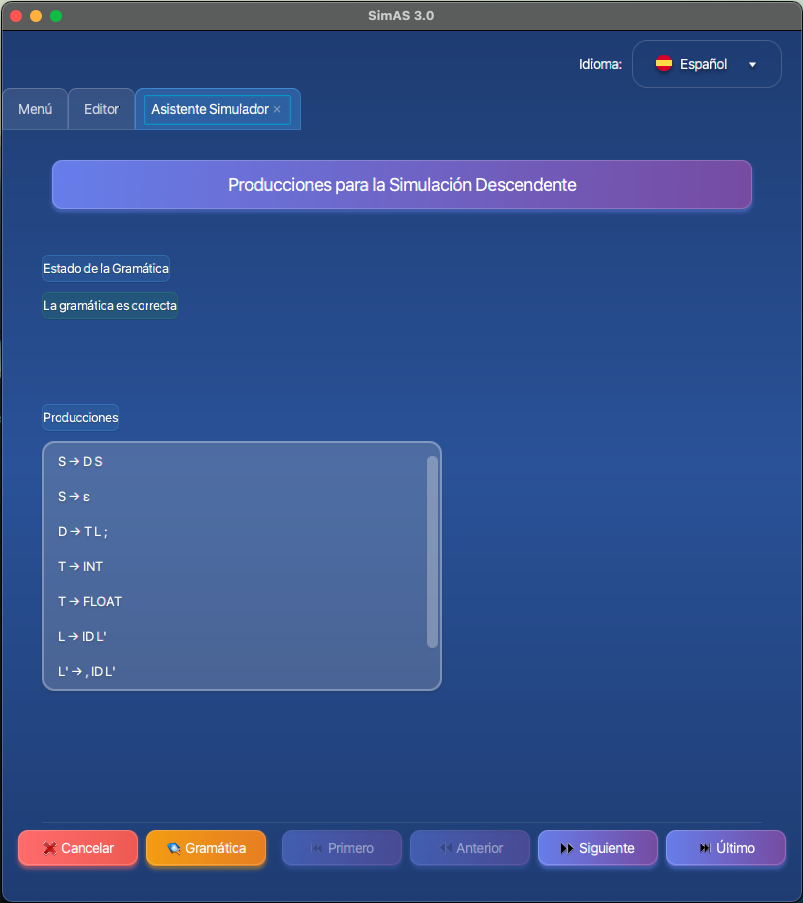
\includegraphics[width=0.9\textwidth]{figuras/simulador/paso1_recursividad_factorizacion.png}
    \caption{Paso 1: Refactorización y eliminación de recursividad}
    \label{fig:paso1_refactorizacion}
\end{figure}

\subsection{Paso 2: Construcción de conjuntos PRIMERO y SIGUIENTE}

El segundo paso representa el núcleo computacional del análisis LL(1), donde el simulador calcula los conjuntos PRIMERO y SIGUIENTE utilizando algoritmos optimizados. Estos conjuntos son fundamentales para la construcción de la tabla predictiva, ya que determinan qué producción aplicar en cada situación durante el análisis.

\subsubsection{Conjunto PRIMERO}

El conjunto PRIMERO de un símbolo $\alpha$, denotado como $PRIMERO(\alpha)$, contiene todos los símbolos terminales que pueden aparecer como primer símbolo en las derivaciones de $\alpha$. El cálculo de PRIMERO es crucial porque determina las condiciones bajo las cuales una producción puede ser aplicada durante el análisis descendente.

El algoritmo implementado maneja casos especiales como:
\begin{itemize}
    \item Símbolos terminales: $PRIMERO(a) = \{a\}$ para cualquier terminal $a$.
    \item Símbolos no terminales: cálculo recursivo considerando todas las producciones.
    \item Cadenas de símbolos: propagación de PRIMERO a través de concatenaciones.
    \item Manejo de $\varepsilon$: inclusión de $\varepsilon$ cuando es derivable.
\end{itemize}

\subsubsection{Conjunto SIGUIENTE}

El conjunto SIGUIENTE de un símbolo no terminal $A$, denotado como $SIGUIENTE(A)$, contiene todos los símbolos terminales que pueden aparecer inmediatamente después de $A$ en alguna derivación desde el símbolo inicial. SIGUIENTE es esencial para manejar producciones que derivan $\varepsilon$.

El algoritmo considera:
\begin{itemize}
    \item El símbolo inicial: $\$ \in SIGUIENTE(S)$ donde $S$ es el símbolo inicial.
    \item Propagación a través de producciones: si $A \rightarrow \alpha B \beta$, entonces $PRIMERO(\beta) \subseteq SIGUIENTE(B)$.
    \item Propagación de $\varepsilon$: si $A \rightarrow \alpha B$ y $\varepsilon \in PRIMERO(\beta)$, entonces $SIGUIENTE(A) \subseteq SIGUIENTE(B)$.
\end{itemize}

\subsubsection{Interfaz del paso 2}

La interfaz del segundo paso, mostrada en la figura \ref{fig:paso2_conjuntos}, presenta los resultados del cálculo de manera clara y organizada:

\begin{itemize}
    \item \textbf{Conjuntos PRIMERO}: presentación tabular de todos los conjuntos PRIMERO calculados para cada símbolo no terminal, con indicadores visuales para símbolos especiales como $\varepsilon$.
    \item \textbf{Conjuntos SIGUIENTE}: visualización completa de todos los conjuntos SIGUIENTE, organizados de manera que facilite la verificación manual y la comprensión de las relaciones entre símbolos.
\end{itemize}

\needspace{8cm}
\begin{figure}[H]
    \centering
    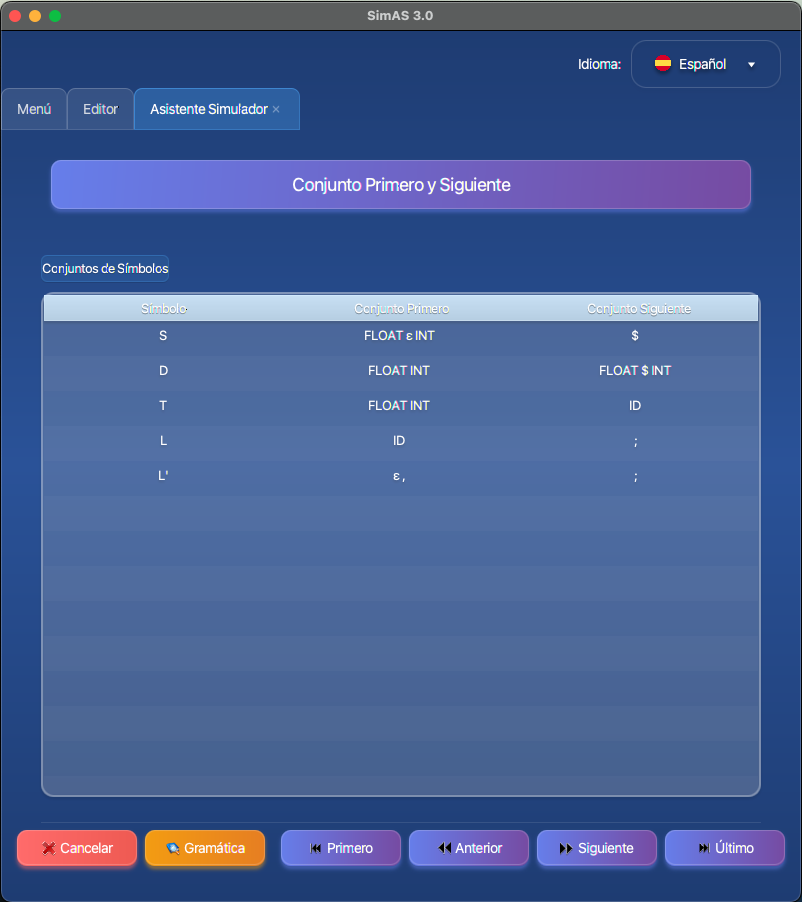
\includegraphics[width=0.9\textwidth]{figuras/simulador/paso2_conjuntos.png}
    \caption{Paso 2: Construcción de conjuntos PRIMERO y SIGUIENTE}
    \label{fig:paso2_conjuntos}
\end{figure}

\subsection{Paso 3: Construcción de la tabla predictiva}

El tercer paso representa la culminación del proceso de preparación, donde el simulador construye la tabla de análisis predictivo utilizando los conjuntos PRIMERO y SIGUIENTE calculados en el paso anterior. Esta tabla es el corazón del analizador LL(1), ya que determina de manera determinista qué acción tomar en cada situación durante el análisis.

\subsubsection{Algoritmo de construcción}

La tabla predictiva $M$ se construye aplicando un algoritmo sistemático que garantiza la corrección y completitud:

\begin{enumerate}
    \item \textbf{Inicialización}: todas las entradas de la tabla se inicializan como vacías.
    \item \textbf{Construcción para cada producción}: para cada producción $A \rightarrow \alpha$:
    \begin{itemize}
        \item Si $a \in PRIMERO(\alpha)$ y $a \neq \varepsilon$, entonces $M[A,a] = A \rightarrow \alpha$.
        \item Si $\varepsilon \in PRIMERO(\alpha)$ y $a \in SIGUIENTE(A)$, entonces $M[A,a] = A \rightarrow \alpha$.
    \end{itemize}
    \item \textbf{Detección de conflictos}: el algoritmo detecta automáticamente conflictos (múltiples producciones para la misma entrada) y los reporta al usuario.
    \item \textbf{Validación LL(1)}: verifica que la tabla resultante define una función total, confirmando que la gramática es LL(1).
\end{enumerate}

\subsubsection{Interfaz del paso 3}

La interfaz del tercer paso, ilustrada en la figura \ref{fig:paso3_tabla_predictiva}, presenta la tabla predictiva de manera intuitiva y educativa:

\begin{itemize}
    \item \textbf{Tabla predictiva completa}: matriz bidimensional que muestra la intersección de símbolos no terminales (filas) y terminales (columnas), con cada celda conteniendo la producción correspondiente o indicando que está vacía.
    \item \textbf{Producciones asignadas}: cada celda no vacía muestra claramente la producción que debe aplicarse, facilitando la comprensión del proceso de análisis y la verificación manual de la corrección.
    \item \textbf{Indicadores visuales}: uso de colores y símbolos para distinguir entre diferentes tipos de entradas y facilitar la identificación de patrones en la tabla.
\end{itemize}

\needspace{8cm}
\begin{figure}[H]
    \centering
    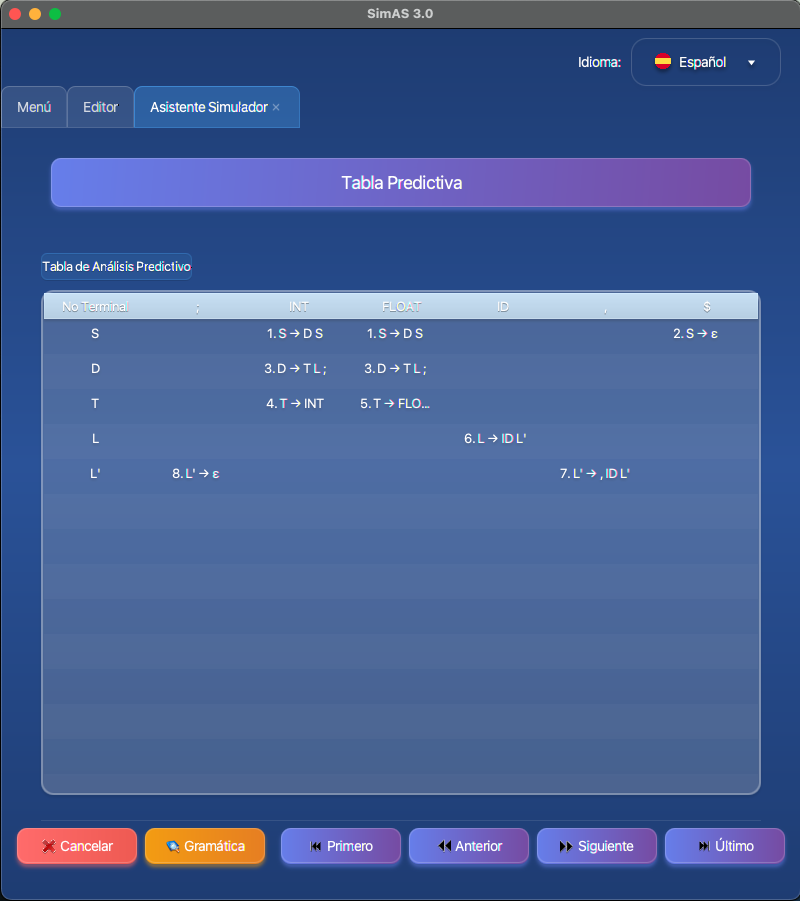
\includegraphics[width=0.9\textwidth]{figuras/simulador/paso3_tablaPredictiva.png}
    \caption{Paso 3: Construcción de la tabla predictiva}
    \label{fig:paso3_tabla_predictiva}
\end{figure}

\subsection{Paso 4: Funciones de error}

El cuarto paso introduce una funcionalidad avanzada que permite configurar un sistema sofisticado de recuperación de errores. Aunque este paso es opcional, su implementación mejora significativamente la experiencia de simulación al proporcionar mecanismos robustos para manejar cadenas de entrada que no pertenecen al lenguaje definido por la gramática.

\subsubsection{Funciones de error del sistema}

El sistema incluye un conjunto predefinido de funciones de error que implementan estrategias estándar de recuperación:

\begin{itemize}
    \item \textbf{Error de inserción}: inserta automáticamente un símbolo terminal esperado en la posición actual, permitiendo que el análisis continúe. Esta función es útil cuando falta un símbolo obligatorio.
    \item \textbf{Error de eliminación}: elimina un símbolo terminal inesperado de la entrada, saltándolo para continuar con el siguiente símbolo. Ideal para manejar símbolos extra o mal posicionados.
    \item \textbf{Error de reemplazo}: reemplaza un símbolo terminal inesperado por otro esperado, manteniendo la posición en la entrada. Útil para correcciones de símbolos similares o errores tipográficos.
\end{itemize}

\subsubsection{Panel de funciones de error}

Al hacer clic en \string"Nueva\string", se abre un panel auxiliar especializado, como se puede observar en las figuras \ref{fig:panel_funciones_error} y \ref{fig:panel_funciones_error_vacio}, que permite:

\begin{itemize}
    \item \textbf{Asignación automática de ID}: el sistema asigna automáticamente el siguiente identificador disponible, garantizando la unicidad y evitando conflictos de nomenclatura.
    \item \textbf{Definición de la función}: interfaz intuitiva para especificar el comportamiento detallado de la función de error, incluyendo condiciones de activación y acciones a realizar.
    \item \textbf{Validación en tiempo real}: verificación automática de que la función definida sea sintácticamente correcta y semánticamente válida antes de permitir su guardado.
    \item \textbf{Guardado seguro}: confirmación y almacenamiento de la función en el sistema, con verificación de integridad y compatibilidad con la gramática actual.
\end{itemize}

\needspace{8cm}
\begin{figure}[H]
    \centering
    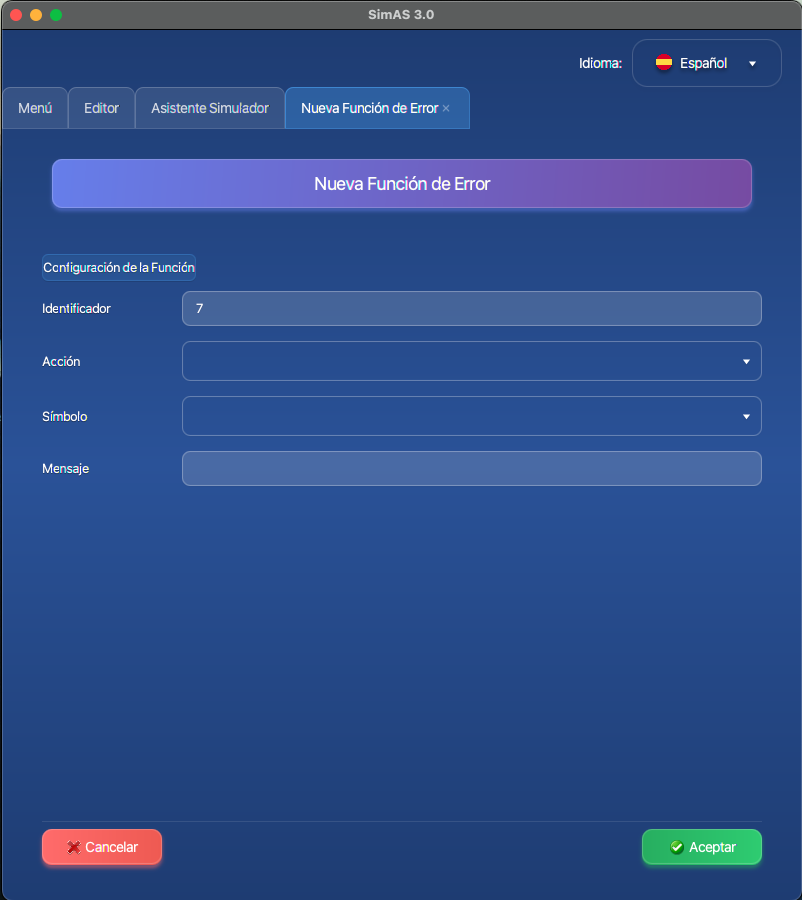
\includegraphics[width=0.9\textwidth]{figuras/simulador/panelFuncError.png}
    \caption{Panel auxiliar para crear nuevas funciones de error}
    \label{fig:panel_funciones_error}
\end{figure}

\needspace{8cm}
\begin{figure}[H]
    \centering
    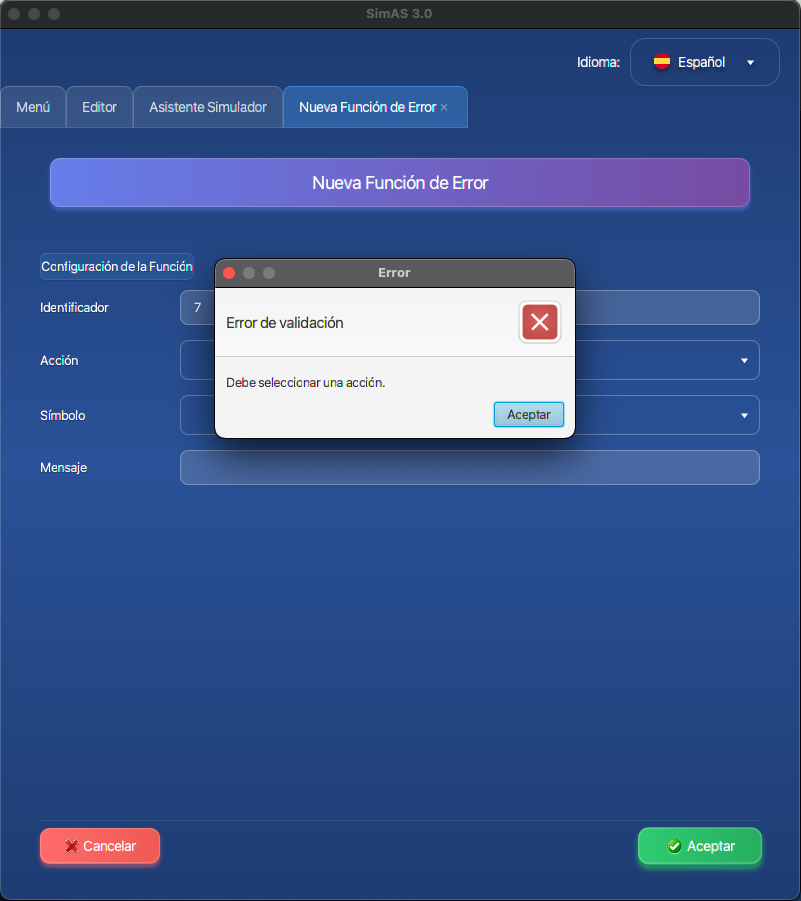
\includegraphics[width=0.9\textwidth]{figuras/simulador/panelFuncError_vacia.png}
    \caption{Panel de funciones de error en estado vacío}
    \label{fig:panel_funciones_error_vacio}
\end{figure}

\subsubsection{Gestión de funciones de error}

El sistema de gestión, ilustrado en las figuras \ref{fig:paso4_funciones_error} y \ref{fig:paso4_sin_funciones_error}, permite al usuario:

\begin{itemize}
    \item \textbf{Añadir nuevas funciones}: capacidad de crear funciones personalizadas de recuperación que se adapten a necesidades específicas o casos de uso particulares.
    \item \textbf{Eliminar funciones}: funcionalidad para quitar funciones no deseadas o que han demostrado ser problemáticas durante las pruebas.
    \item \textbf{Omitir funciones de error}: opción de continuar sin sistema de recuperación para análisis más estrictos o cuando se desea que el analizador falle inmediatamente ante errores.
\end{itemize}

\needspace{8cm}
\begin{figure}[H]
    \centering
    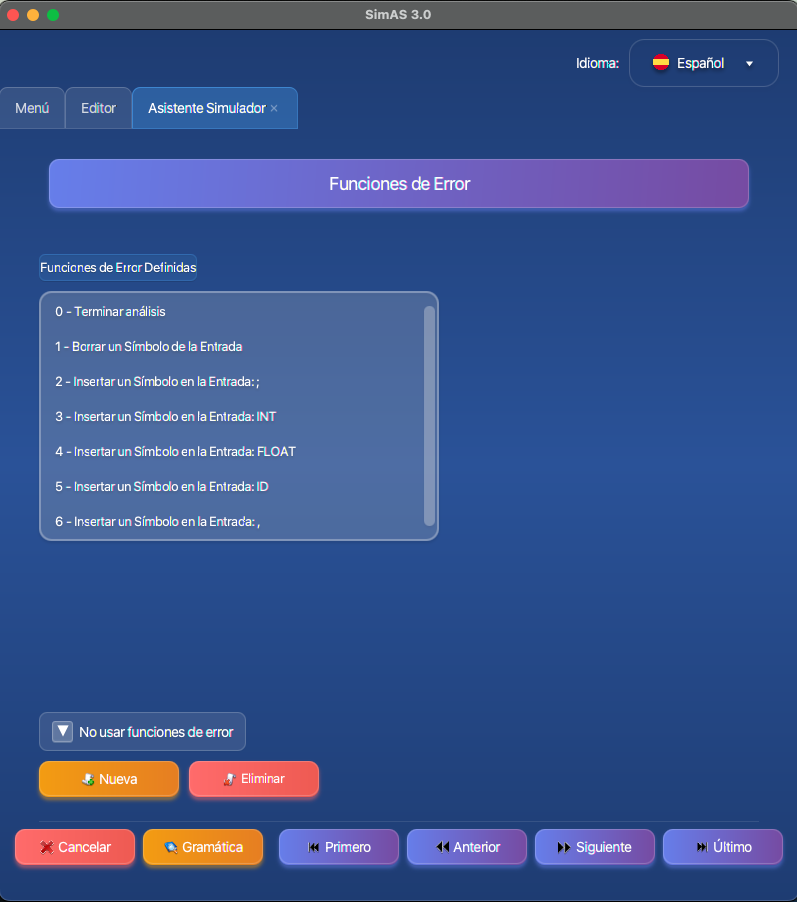
\includegraphics[width=0.9\textwidth]{figuras/simulador/paso4_funcionesError.png}
    \caption{Paso 4: Configuración de funciones de error}
    \label{fig:paso4_funciones_error}
\end{figure}

\needspace{8cm}
\begin{figure}[H]
    \centering
    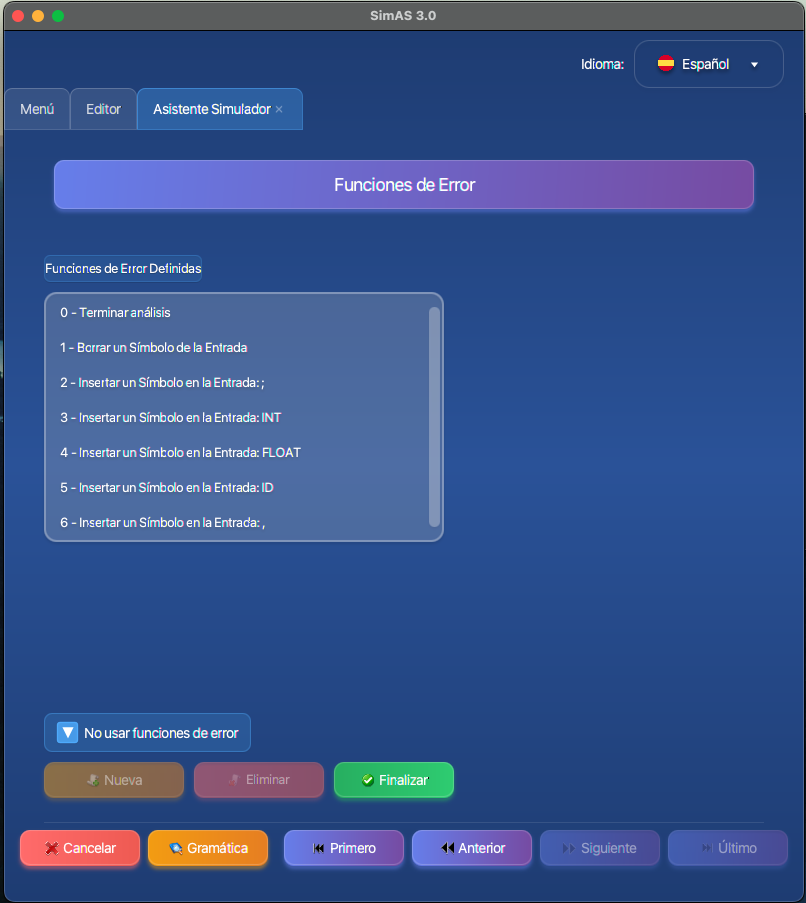
\includegraphics[width=0.9\textwidth]{figuras/simulador/paso4_no_usar_funError.png}
    \caption{Paso 4: Opción de no usar funciones de error}
    \label{fig:paso4_sin_funciones_error}
\end{figure}

\subsection{Paso 5: Tabla predictiva completa}

El quinto y último paso del asistente presenta la tabla predictiva final en su forma completa, integrando todas las producciones calculadas con las funciones de error configuradas. Este paso proporciona al usuario la oportunidad de realizar ajustes finales y personalizaciones antes de proceder con la simulación, asegurando que la configuración sea exactamente como se desea.

\subsubsection{Interfaz del paso 5}

La interfaz del paso final, mostrada en la figura \ref{fig:paso5_tabla_completa}, presenta una vista comprensiva y editable de la tabla predictiva:

\begin{itemize}
    \item \textbf{Tabla predictiva completa}: visualización integral que combina todas las producciones calculadas con las funciones de error configuradas, proporcionando una vista unificada del comportamiento del analizador.
    \item \textbf{Celdas editables interactivas}: cada celda de la tabla es clickeable, permitiendo al usuario añadir, modificar o eliminar funciones de error en posiciones específicas según sus necesidades.
    \item \textbf{Herramientas de edición avanzadas}: conjunto completo de herramientas para modificar la tabla, incluyendo operaciones de edición masiva y validación en tiempo real.
    \item \textbf{Vista previa en tiempo real}: representación visual que se actualiza instantáneamente con cada modificación, permitiendo al usuario verificar inmediatamente el impacto de sus cambios.
\end{itemize}

\needspace{8cm}
\begin{figure}[H]
    \centering
    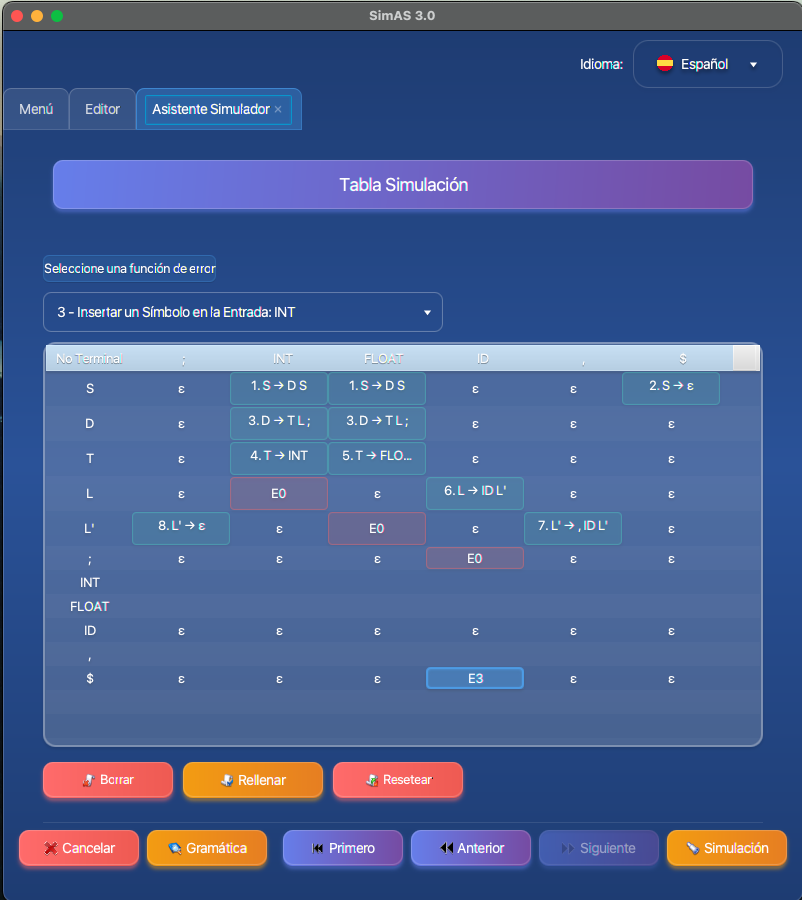
\includegraphics[width=0.9\textwidth]{figuras/simulador/paso5_tablaPredictivaCompleta.png}
    \caption{Paso 5: Tabla predictiva completa con herramientas de edición}
    \label{fig:paso5_tabla_completa}
\end{figure}

\subsubsection{Herramientas de edición}

El paso 5 incorpora un conjunto sofisticado de herramientas de edición diseñadas para facilitar la personalización de la tabla:

\begin{itemize}
    \item \textbf{Borrar selectivo}: elimina el contenido de una celda seleccionada, restringido únicamente a funciones de error para preservar la integridad de las producciones fundamentales.
    \item \textbf{Resetear a estado original}: restaura la tabla a su configuración inicial, manteniendo solo las producciones básicas y eliminando todas las funciones de error añadidas.
    \item \textbf{Rellenar con epsilon}: llena las celdas vacías con símbolos epsilon para mejorar la legibilidad visual, aunque esta operación es puramente cosmética.
\end{itemize}

\section{Simulador principal}

Una vez completados exitosamente los 5 pasos del asistente, el usuario accede al simulador principal, que representa el núcleo operativo del sistema. Esta transición se realiza mediante el botón \string"Simulación\string", que activa el entorno de simulación con toda la configuración previamente establecida.

\subsection{Interfaz del simulador}

El simulador principal, ilustrado en la figura \ref{fig:simulador_principal}, presenta una interfaz diseñada para proporcionar acceso inmediato a todas las funcionalidades esenciales:

\begin{itemize}
    \item \textbf{Resumen de configuración}: panel comprensivo que muestra las producciones modificadas, las funciones de error configuradas y la tabla predictiva final, proporcionando una vista de conjunto de toda la configuración.
    \item \textbf{Botón \string"Informe\string"}: genera automáticamente un informe PDF detallado que documenta toda la configuración y los resultados del proceso de preparación.
    \item \textbf{Botón \string"Simular\string"}: inicia el proceso de simulación interactiva, abriendo una nueva pestaña dedicada al análisis sintáctico.
\end{itemize}

\needspace{8cm}
\begin{figure}[H]
    \centering
    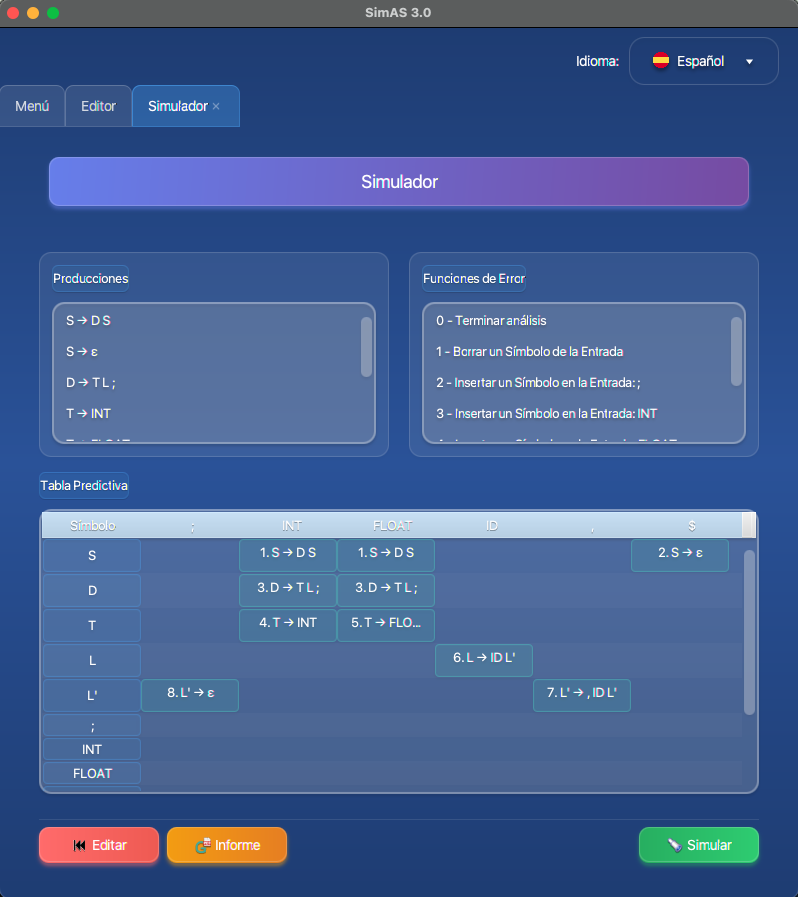
\includegraphics[width=0.9\textwidth]{figuras/simulador/simulador.png}
    \caption{Interfaz del simulador principal}
    \label{fig:simulador_principal}
\end{figure}

\subsection{Generación de informes}

El sistema de generación de informes representa una funcionalidad avanzada que produce documentación profesional y completa. El botón \string"Informe\string" genera un documento PDF estructurado que incluye:

\begin{itemize}
    \item \textbf{Información del editor}: documentación completa de la gramática original y todas las modificaciones aplicadas durante el proceso de refactorización.
    \item \textbf{Conjuntos PRIMERO y SIGUIENTE}: presentación detallada de todos los conjuntos calculados en el paso 2, con explicaciones de su significado y uso.
    \item \textbf{Tabla predictiva}: representación completa de la tabla final, incluyendo todas las producciones y funciones de error integradas.
    \item \textbf{Funciones de error}: documentación exhaustiva de todas las funciones de error configuradas, incluyendo sus definiciones, comportamientos y casos de uso.
    \item \textbf{Estadísticas y métricas}: análisis cuantitativo de la gramática y la configuración, incluyendo métricas de complejidad, cobertura y eficiencia.
\end{itemize}

\section{Simulación interactiva}

La simulación interactiva representa el corazón de la experiencia educativa de SimAS 3.0. Al hacer clic en \string"Simular\string", se abre una nueva pestaña especializada que proporciona un entorno completo para realizar análisis sintáctico con control total del usuario sobre cada aspecto del proceso.

\subsection{Interfaz de simulación}

La pestaña de simulación, mostrada en las figuras \ref{fig:simulacion_vacia} y \ref{fig:simulacion_cadena_entrada}, incorpora una interfaz intuitiva y funcional que incluye:

\begin{itemize}
    \item \textbf{Campo de entrada inteligente}: área de texto especializada para introducir la cadena a analizar, con validación en tiempo real y sugerencias de símbolos válidos.
    \item \textbf{Símbolos disponibles}: panel que muestra todos los símbolos terminales válidos para la gramática actual, facilitando la construcción de cadenas de entrada correctas.
    \item \textbf{Controles de simulación avanzados}: conjunto completo de botones para iniciar, pausar, reanudar y controlar granularmente la simulación.
    \item \textbf{Historial de pasos detallado}: registro comprensivo de cada paso del análisis, incluyendo estados intermedios y decisiones tomadas.
    \item \textbf{Navegación bidireccional}: botones para avanzar y retroceder en los pasos, permitiendo revisar y analizar cualquier momento del proceso.
\end{itemize}

\needspace{8cm}
\begin{figure}[H]
    \centering
    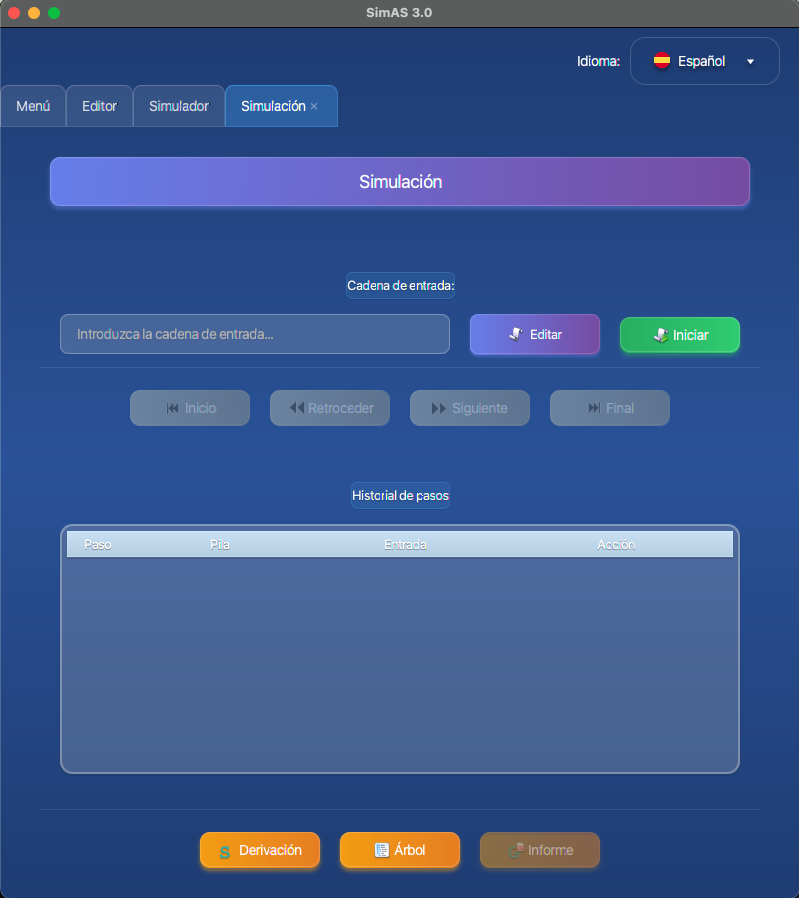
\includegraphics[width=0.9\textwidth]{figuras/simulador/simulacion_vacia.png}
    \caption{Interfaz de simulación en estado vacío}
    \label{fig:simulacion_vacia}
\end{figure}

\needspace{8cm}
\begin{figure}[H]
    \centering
    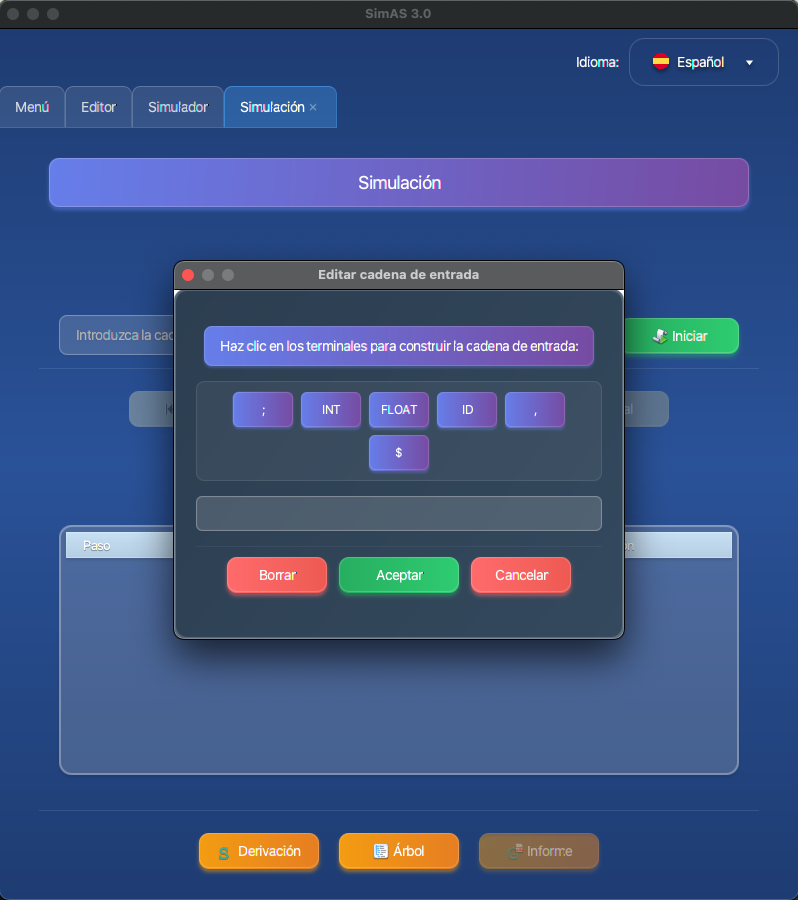
\includegraphics[width=0.9\textwidth]{figuras/simulador/simulacion_cadenaEntrada.png}
    \caption{Interfaz de simulación con cadena de entrada}
    \label{fig:simulacion_cadena_entrada}
\end{figure}

\subsection{Proceso de simulación}

El proceso de simulación implementa un algoritmo LL(1) completo que sigue una secuencia estructurada:

\begin{enumerate}
    \item \textbf{Entrada y validación de cadena}: el usuario introduce la cadena a analizar, y el sistema valida que contenga únicamente símbolos terminales válidos para la gramática.
    \item \textbf{Inicialización del analizador}: se configura la pila de análisis con el símbolo inicial y se prepara el entorno de simulación.
    \item \textbf{Ejecución del algoritmo LL(1)}: el analizador procesa la cadena utilizando la tabla predictiva, aplicando producciones y funciones de error según sea necesario.
    \item \textbf{Control interactivo}: el usuario mantiene control total sobre el avance de la simulación, pudiendo pausar, avanzar paso a paso o retroceder en cualquier momento.
    \item \textbf{Resultado final}: el sistema determina si la cadena es aceptada o rechazada, proporcionando detalles completos del proceso y estadísticas del análisis.
\end{enumerate}

\subsection{Historial de pasos}

El sistema de historial, ilustrado en la figura \ref{fig:simulacion_completa}, proporciona una vista detallada de cada paso del análisis:

\begin{itemize}
    \item \textbf{Pila de análisis}: representación visual del estado actual de la pila, mostrando los símbolos pendientes de procesar.
    \item \textbf{Acción aplicada}: documentación clara de la producción o función de error utilizada en cada paso, con justificación de la decisión.
    \item \textbf{Estado del análisis}: información comprensiva sobre el progreso actual, incluyendo posición en la entrada y estado de la pila.
    \item \textbf{Métricas de rendimiento}: estadísticas en tiempo real sobre el número de pasos, eficiencia del análisis y uso de funciones de error.
\end{itemize}

\needspace{8cm}
\begin{figure}[H]
    \centering
    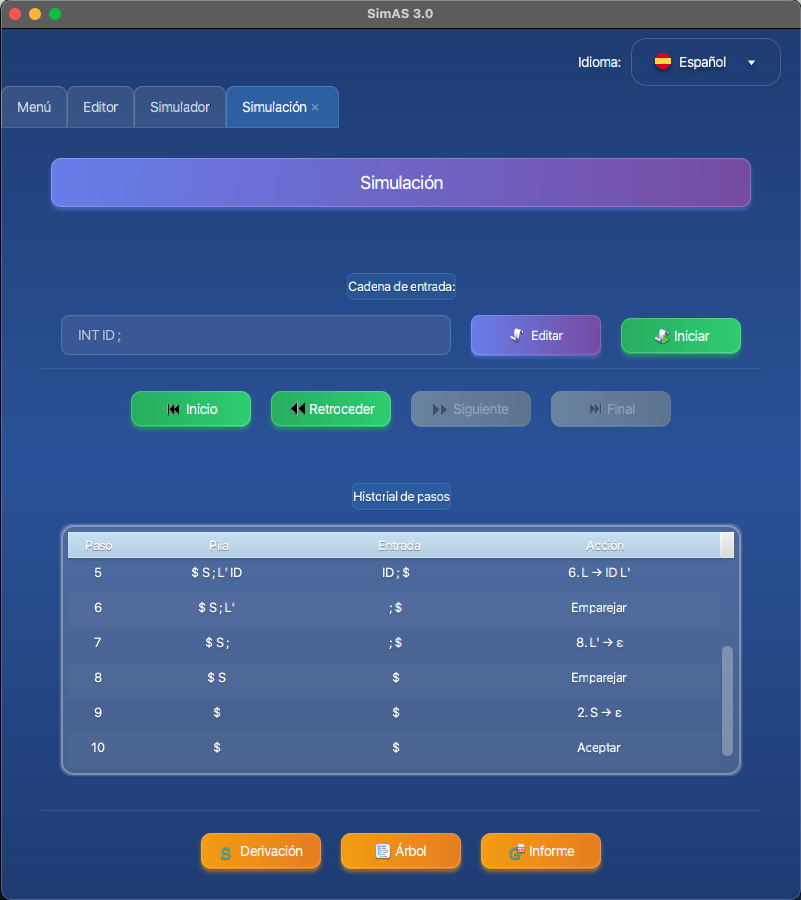
\includegraphics[width=0.9\textwidth]{figuras/simulador/simulacion_completa.png}
    \caption{Simulación completa con historial de pasos}
    \label{fig:simulacion_completa}
\end{figure}

\subsection{Navegación en la simulación}

El sistema de navegación proporciona control granular sobre la simulación:

\begin{itemize}
    \item \textbf{Avance paso a paso}: ejecuta un único paso del análisis, permitiendo al usuario examinar cada decisión en detalle.
    \item \textbf{Retroceso inteligente}: permite volver al paso anterior manteniendo la integridad del estado de la simulación.
    \item \textbf{Finalización automática}: salta al final de la simulación para obtener el resultado inmediatamente.
    \item \textbf{Reinicio completo}: restaura la simulación a su estado inicial, permitiendo comenzar de nuevo con la misma cadena o una nueva.
\end{itemize}

\section{Visualización de resultados}

El simulador incorpora un sistema avanzado de visualización que proporciona dos tipos complementarios de representación que se actualizan dinámicamente durante la simulación, facilitando la comprensión del proceso de análisis sintáctico.

\subsection{Derivación}

La derivación muestra la secuencia de producciones aplicadas durante el análisis, como se puede observar en la figura \ref{fig:simulacion_derivacion}:

\begin{itemize}
    \item \textbf{Acceso directo}: botón \string"Derivación\string" en la pestaña de simulación que abre una nueva pestaña dedicada.
    \item \textbf{Actualización automática}: se actualiza en tiempo real conforme avanza la simulación, mostrando cada paso de derivación.
    \item \textbf{Formato BNF estándar}: representación clara y estándar de cada paso de derivación, facilitando la comprensión del proceso.
    \item \textbf{Navegación sincronizada}: los cambios en la derivación reflejan exactamente la posición actual en la simulación, manteniendo la coherencia.
\end{itemize}

\needspace{8cm}
\begin{figure}[H]
    \centering
    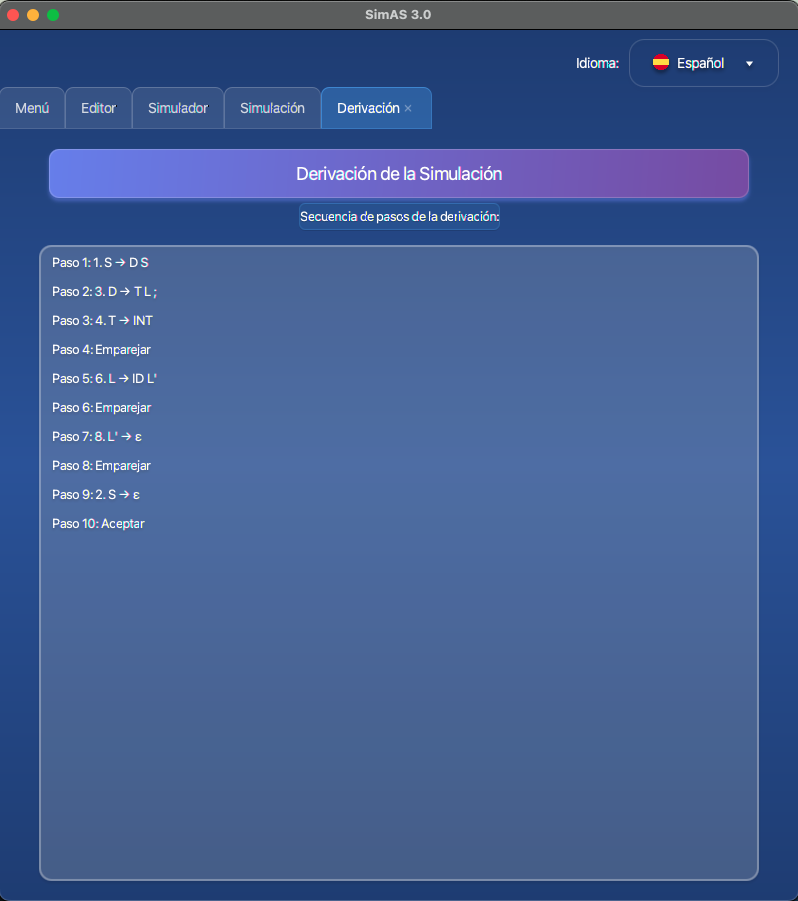
\includegraphics[width=0.9\textwidth]{figuras/simulador/simulacion_derivacion.png}
    \caption{Vista de la derivación durante la simulación}
    \label{fig:simulacion_derivacion}
\end{figure}

\subsection{Árbol sintáctico}

El árbol sintáctico proporciona una representación visual de la estructura de la cadena, ilustrado en la figura \ref{fig:simulacion_arbol}:

\begin{itemize}
    \item \textbf{Acceso directo}: botón \string"Árbol\string" en la pestaña de simulación que abre una nueva pestaña dedicada.
    \item \textbf{Construcción progresiva}: se construye paso a paso durante la simulación, mostrando el crecimiento del árbol en tiempo real.
    \item \textbf{Representación gráfica avanzada}: estructura jerárquica clara y legible con elementos visuales que facilitan la comprensión.
    \item \textbf{Sincronización perfecta}: refleja exactamente el estado actual de la simulación, manteniendo la coherencia con la derivación.
\end{itemize}

\needspace{8cm}
\begin{figure}[H]
    \centering
    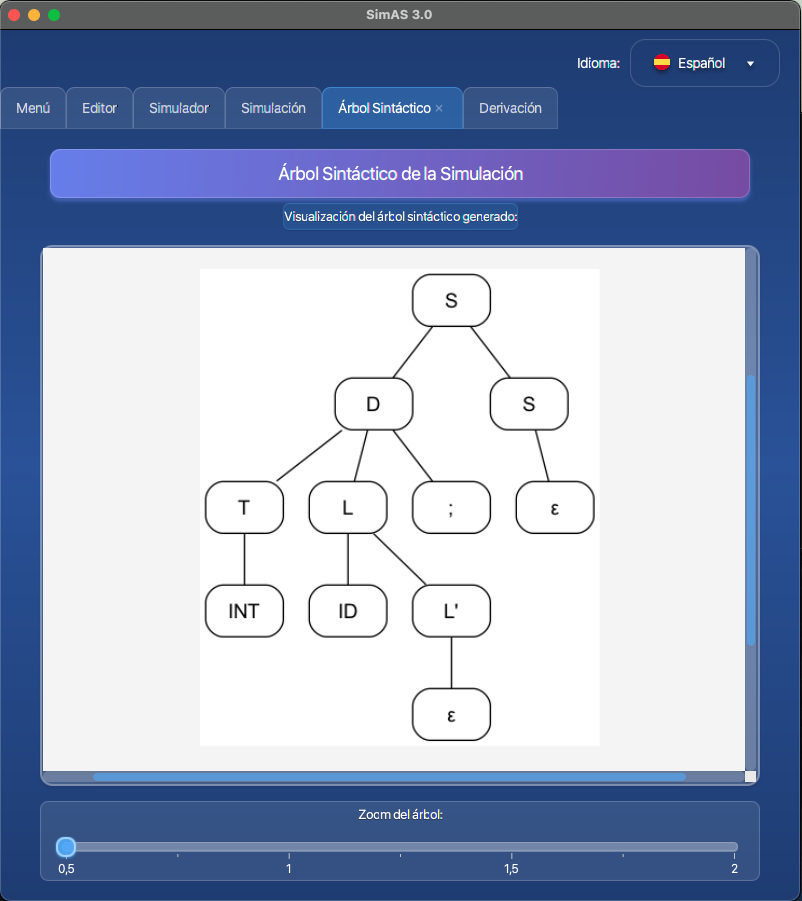
\includegraphics[width=0.9\textwidth]{figuras/simulador/simulacion_arbol.png}
    \caption{Vista del árbol sintáctico durante la simulación}
    \label{fig:simulacion_arbol}
\end{figure}

\section{Múltiples simulaciones}

Una característica avanzada y distintiva del simulador es la capacidad de manejar múltiples simulaciones simultáneamente, proporcionando una experiencia de análisis comparativo y exhaustivo que no se encuentra en herramientas similares.

\subsection{Gestión de simulaciones}

Para cada configuración de simulador, el sistema permite una gestión sofisticada:

\begin{itemize}
    \item \textbf{Crear nuevas simulaciones}: capacidad de simular diferentes cadenas de entrada manteniendo la misma configuración de gramática y funciones de error.
    \item \textbf{Mantener simulaciones activas}: múltiples simulaciones pueden estar abiertas simultáneamente, cada una en su propia pestaña independiente.
    \item \textbf{Comparar resultados}: análisis comparativo de diferentes cadenas con la misma gramática, facilitando la identificación de patrones y comportamientos.
    \item \textbf{Gestión independiente}: cada simulación mantiene su propio estado, historial y visualizaciones, permitiendo análisis paralelos sin interferencias.
\end{itemize}

\subsection{Ventajas de múltiples simulaciones}

Esta funcionalidad avanzada, mostrada en la figura \ref{fig:simulacion_varias}, permite:

\begin{itemize}
    \item \textbf{Análisis comparativo avanzado}: probar diferentes cadenas con la misma gramática, facilitando la identificación de patrones y comportamientos específicos.
    \item \textbf{Validación exhaustiva}: verificar el comportamiento del analizador con múltiples casos de prueba, incluyendo casos límite y escenarios complejos.
    \item \textbf{Experimentos educativos}: explorar diferentes escenarios de análisis, permitiendo a los estudiantes comprender mejor los conceptos teóricos.
    \item \textbf{Eficiencia operativa}: no es necesario reconfigurar el simulador para cada nueva cadena, optimizando el flujo de trabajo y la productividad.
\end{itemize}

\needspace{8cm}
\begin{figure}[H]
    \centering
    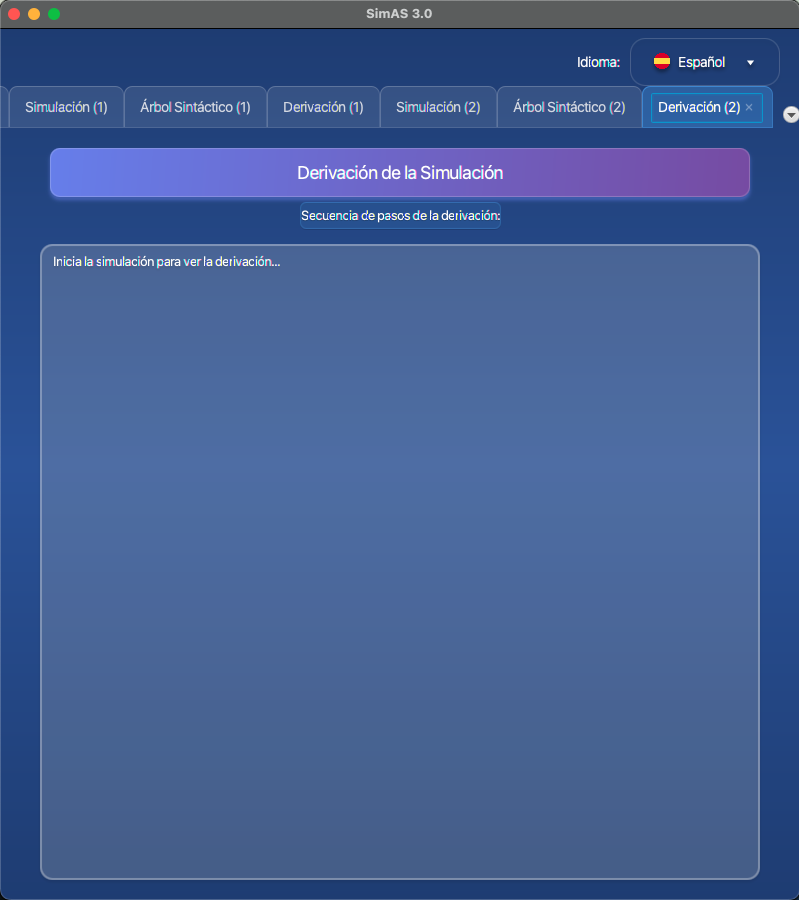
\includegraphics[width=0.9\textwidth]{figuras/simulador/simulacion_varias.png}
    \caption{Ejemplo de múltiples simulaciones simultáneas}
    \label{fig:simulacion_varias}
\end{figure}

\section{Integración con el editor}

El simulador mantiene una integración profunda y transparente con el editor de gramáticas, creando un flujo de trabajo unificado y eficiente:

\begin{itemize}
    \item \textbf{Transición automática}: paso directo y sin interrupciones del editor al simulador, manteniendo toda la configuración y estado.
    \item \textbf{Sincronización de datos en tiempo real}: cambios realizados en el editor se reflejan inmediatamente en el simulador, garantizando la coherencia.
    \item \textbf{Consistencia garantizada}: el sistema asegura que la gramática simulada es exactamente la misma que la editada, eliminando errores de configuración.
    \item \textbf{Flujo de trabajo optimizado}: proceso continuo y fluido desde la creación y edición de gramáticas hasta su simulación y análisis.
\end{itemize}

\section{Resolución de problemas}

El simulador incluye un sistema robusto de detección y resolución de problemas que ayuda a los usuarios a identificar y solucionar dificultades comunes durante el proceso de simulación.

\subsection{Problemas comunes}

El sistema está diseñado para manejar y resolver automáticamente los siguientes problemas típicos:

\begin{itemize}
    \item \textbf{Gramática no LL(1)}: el sistema detecta automáticamente conflictos en la tabla predictiva y proporciona sugerencias específicas para resolverlos.
    \item \textbf{Recursividad no eliminable}: se informa al usuario sobre limitaciones estructurales y se sugieren alternativas de diseño.
    \item \textbf{Funciones de error incorrectas}: validación automática previene errores de configuración y proporciona retroalimentación detallada.
    \item \textbf{Cadenas inválidas}: el sistema valida la entrada antes de la simulación y proporciona información específica sobre símbolos no válidos.
\end{itemize}

\subsection{Soluciones recomendadas}

Para resolver problemas comunes, se recomiendan las siguientes estrategias:

\begin{itemize}
    \item \textbf{Revisar la gramática}: verificar que la gramática sea LL(1) utilizando las herramientas de validación del editor.
    \item \textbf{Ajustar funciones de error}: modificar o eliminar funciones problemáticas utilizando el panel de gestión del paso 4.
    \item \textbf{Validar entrada}: asegurar que la cadena contenga únicamente símbolos terminales válidos para la gramática actual.
    \item \textbf{Consultar la documentación}: revisar ejemplos y casos de uso para comprender mejor el comportamiento esperado.
\end{itemize}

\section{Conclusión}

El simulador de análisis sintáctico descendente predictivo de SimAS 3.0 representa una herramienta educativa de vanguardia que combina la potencia algorítmica del análisis LL(1) con una interfaz intuitiva y educativa de última generación. El asistente guiado de 5 pasos simplifica significativamente la configuración compleja requerida para el análisis sintáctico, mientras que las funciones avanzadas de visualización y múltiples simulaciones proporcionan una experiencia de aprendizaje rica, completa y profundamente educativa.

La integración perfecta y transparente con el editor de gramáticas, el sistema avanzado de recuperación de errores, y la capacidad de generar informes detallados y profesionales hacen del simulador una herramienta indispensable para el estudio, la práctica y la investigación del análisis sintáctico. La funcionalidad innovadora de múltiples simulaciones permite una exploración exhaustiva y comparativa de las capacidades de la gramática, mientras que la navegación paso a paso y las visualizaciones dinámicas facilitan la comprensión profunda de los conceptos teóricos subyacentes.

El simulador no solo demuestra la corrección y eficiencia de las gramáticas, sino que también educa de manera integral sobre el proceso completo de análisis sintáctico, proporcionando una base sólida y comprensiva para el aprendizaje de conceptos avanzados en teoría de lenguajes formales, compiladores y análisis sintáctico. Su diseño educativo y su implementación técnica robusta lo convierten en una herramienta de referencia para la enseñanza y el aprendizaje de estos conceptos fundamentales en ciencias de la computación.

